\documentclass[12pt,a4paper,preprint]{elsarticle}
\usepackage[T2A]{fontenc}
\usepackage[utf8]{inputenc}
\usepackage[russian]{babel}
\usepackage[a4paper,left=2cm,right=2cm,top=2cm,bottom=2.7cm]{geometry}
\usepackage{amsmath,amssymb,amsfonts,amsthm,bm,graphicx,booktabs,multirow,array,tabularx,xcolor,hyperref}

\makeatletter
\def\ps@pprintTitle{%
    \let\@mkboth\markboth
    \def\@evenhead{%
        \ifnum\c@page>1
            {\footnotesize\thepage}\hfil{\footnotesize\itshape\leftmark}%
        \fi}%
    \def\@oddfoot{\footnotesize\itshape
        Preprint\hfill\thepage\relax}%
    \let\@evenfoot\@oddfoot
}
\AtBeginDocument{\pagestyle{pprintTitle}}
\makeatother
\graphicspath{{figs/}}

\begin{document}
    \begin{frontmatter}
        \title{Макроскопическое квантовое туннелирование между\\акустическими чёрной и белой дырами в потоке Мишеля}
        \author{Alexander V. Semyannikov}
        \address{Independent Researcher \\ \textit{Email: avsemyannikov@gmail.com}}
        
        \begin{abstract}
            Релятивистский поток Мишеля обладает двумя вырожденными стационарными решениями: аккреционной ветвью ($\upsilon < 0$), формирующей акустическую чёрную дыру, и ветровой ветвью ($\upsilon > 0$), формирующей акустическую белую дыру. Оба решения являются стационарными точками одного энергетического функционала; барьер между ними имеет инерционную природу и обусловлен необходимостью остановки и разворота макроскопического потока. В рамках однопараметрической модельной редукции построена инстантонная траектория в евклидовом времени, соединяющая две ветви через седловую точку фазового пространства. Инстантонное действие выражается через эффективный момент инерции потока и высоту энергетического барьера; оба множителя конечны благодаря сходимости интеграла с фактором $\upsilon^{2}$. Численные оценки для $a_{\infty} \in \{0{,}05;\, 0{,}1\}$ показывают, что инстантонное действие контролируется макроскопическими масштабами акустического горизонта. Вероятность перехода экспоненциально подавлена и приобретает физический смысл только для систем с квантовой микроструктурой ($\hbar_{\mathrm{eff}} > 0$). Детальный баланс между прямым и обратным переходами нарушен вследствие классической неустойчивости акустической белой дыры. Конструкция согласована с инвариантными величинами, установленными в сопутствующих исследованиях.
        \end{abstract}
        
        \begin{keyword}
            аккреция Мишеля \sep аналоговая гравитация \sep акустическая чёрная дыра \sep акустическая белая дыра \sep макроскопическое квантовое туннелирование \sep инстантон \sep координаты Пенлеве--Гульстранда \sep поверхностная гравитация \sep излучение Хокинга \sep конденсат Бозе--Эйнштейна
        \end{keyword}
    \end{frontmatter}

    \section{Введение}\label{sec:introduction}
        Акустические возмущения в движущейся жидкости распространяются на эффективной лоренцевой геометрии, построенной из фоновой метрики пространства-времени, 4-скорости потока и локальной скорости звука~\cite{UnruhWG_ExperimentalBlackHoleEvaporation_1981, VisserM_AcousticBlackHolesHorizonsErgospheresAndHawkingRadiation_1998, BarceloC_LiberatiS_VisserM_AnalogueGravity_2011}. Для стационарной сферической аккреции на чёрную дыру Шварцшильда --- потока Мишеля~\cite{MichelFC_AccretionOfMatterByCondensedObjects_1972} --- эта конструкция порождает акустический горизонт, совпадающий с критической точкой потока~\cite{SemyannikovAV_AcousticGeometryAndSoundRayDynamicsInRelativisticSphericalAccretion_2026}. Геометрико-оптическая феноменология звуковых лучей во внешней дозвуковой области построена в~\cite{SemyannikovAV_AcousticGeometryAndSoundRayDynamicsInRelativisticSphericalAccretion_2026}; спектр конечно-частотных возмущений и регуляризация пространственной задачи акустическим горизонтом установлены в~\cite{SemyannikovAV_PerturbationSpectrumOfMichelFlowAcousticVorticalAndEntropyModes_2026}; глобальная PG-конструкция, регулярная на обоих горизонтах, развита в~\cite{SemyannikovAV_GlobalAcousticGeometryOfMichelFlowInPainleveGullstrandCoordinates_2026}.
        
        Структурно параллельное направление исследований, наиболее явно развиваемое Воловиком~\cite{VolovikGE_PainleveGullstrandCoordinatesForSchwarzschildDeSitterSpacetime_2023}, обращается к соотношению между состояниями чёрной и белой дыр в рамках единого формализма. В расширенном описании пространства-времени Шварцшильда--де~Ситтера в координатах Пенлеве--Гульстранда (PG) функция сдвига меняет знак в стационарной точке, а девять реализаций конфигурации --- включая чёрные и белые дыры, сжимающиеся и расширяющиеся космологии --- оказываются связанными сингулярными преобразованиями координат на горизонтах. Эти преобразования, хотя и сингулярны лишь координатно, интерпретируются как описывающие макроскопическое квантовое туннелирование между физически неэквивалентными вакуумными состояниями, причём экспонента туннелирования связана с разностью их энтропий. Переход от чёрной дыры к белой тем самым формулируется как топологический квантовый процесс, а не как неустойчивость единственного классического решения.
        
        Поток Мишеля несёт точный гидродинамический аналог этой структуры. Стационарное трансзвуковое решение выделяется одновременным обращением в нуль числителя и знаменателя $\mathrm{d}\upsilon/\mathrm{d}r$, что идентифицирует звуковую точку как седло в фазовой плоскости $(\upsilon, r)$. Аккреционная ветвь, $\upsilon < 0$, плавно переходит от дозвуковых условий на бесконечности к сверхзвуковым у горизонта и порождает акустическую чёрную дыру; ветровая ветвь, $\upsilon > 0$, проходит через то же седло в противоположном направлении и порождает акустическую белую дыру. Обе ветви имеют тождественные интегралы движения и тождественные термодинамические параметры, однако они разделены классически запрещённой областью: любая непрерывная эволюция от одной ветви к другой потребовала бы от жидкости бесконечно долго задерживаться в седловой точке. Это разделение является гидродинамическим аналогом дихотомии чёрной и белой дыр в вакуумной гравитации.
        
        В настоящей работе формулируется и оценивается макроскопическое квантовое туннелирование между состояниями акустической чёрной и акустической белой дыр в потоке Мишеля. Представление PG, развитое в~\cite{SemyannikovAV_GlobalAcousticGeometryOfMichelFlowInPainleveGullstrandCoordinates_2026}, расширяется на обе ветви в рамках единой гладкой координатной карты, а инстантонное действие, управляющее переходом, выражается через гидродинамические переменные потока. Экспонента туннелирования связывается с формальной площадью акустического горизонта и с поверхностной гравитацией $\kappa$, тем самым соединяя макроскопический переход с кинематическим масштабом Хокинга, установленным в предыдущих работах. Результат представляет собой количественную реализацию --- в рамках релятивистской гидродинамики --- механизма туннелирования между чёрной и белой дырами, изначально предложенного для вакуумных пространств-времён.

    \section{Дуализм аккреции и ветра и седловая структура потока Мишеля}\label{sec:duality}
        На протяжении работы используется система единиц $G = c = 1$; длины безразмерны и измеряются в единицах гравитационного радиуса $r_{\mathrm{g}}$; скорости и скорость звука --- в единицах $c$; термодинамические переменные нормированы на свои асимптотические значения в системе покоя в соответствии со стандартной конвенцией для потока Мишеля~\cite{MichelFC_AccretionOfMatterByCondensedObjects_1972, MoncriefV_StabilityOfStationarySphericalAccretionOntoASchwarzschildBlackHole_1980}; индексы «$\infty$», «c», «g» и «a» обозначают асимптотику на бесконечности, критическую точку, гравитационный и акустический горизонты соответственно.
        \subsection{Интегралы Мишеля и критическая точка}\label{subsec:michel-integrals}
            Фоновое пространство-время описывается метрикой Шварцшильда
            \begin{equation}
                \mathrm{d}s^{2} = -f\,\mathrm{d}t^{2} + f^{-1}\,\mathrm{d}r^{2} + r^{2}\bigl(\mathrm{d}\theta^{2}+\sin^{2}\theta\,\mathrm{d}\phi^{2}\bigr), \qquad f(r) = 1 - \frac{1}{r},
                \label{eq:schwarzschild-metric}
            \end{equation}
            с гравитационным горизонтом при $r = 1$. Стационарное сферически-симметричное течение совершенной жидкости~\cite{MichelFC_AccretionOfMatterByCondensedObjects_1972} характеризуется 4-скоростью
            \begin{equation}
                u^{\mu} = (\vartheta,\,\upsilon,\,0,\,0), \qquad f\vartheta = \sqrt{f + \upsilon^{2}}, \qquad \upsilon < 0,
                \label{eq:four-velocity}
            \end{equation}
            где $\vartheta$ --- временная компонента, $\upsilon$ --- радиальная 3-скорость, а условие $\upsilon < 0$ выделяет ветвь аккреции. Фон фиксируется двумя первыми интегралами, где $n$ --- концентрация частиц, $h$ --- удельная энтальпия, а $\mathcal{J}$ --- поток барионов:
            \begin{equation}
                r^{2} n \upsilon = \mathcal{J}, \qquad h\sqrt{f + \upsilon^{2}} = h_{\infty}.
                \label{eq:michel-integrals}
            \end{equation}
            Первый интеграл выражает сохранение потока барионов через сферическую поверхность, второй --- сохранение удельной энергии вдоль линии тока и служит релятивистским аналогом уравнения Бернулли. Эти соотношения совместно с политропным уравнением состояния $p = K n^{\gamma}$ определяют гидродинамические профили $\upsilon(r)$ и $a(r)$ для заданных показателя адиабаты $\gamma$ и асимптотической скорости звука $a_{\infty}$.
            
            Плавный трансзвуковой переход через критическую точку $r_{\mathrm{c}}$ требует одновременного обращения в нуль числителя и знаменателя $\mathrm{d}\upsilon/\mathrm{d}r$, что даёт стандартные условия~\cite{ShapiroSL_TeukolskySA_BlackHolesWhiteDwarfsAndNeutronStarsThePhysicsOfCompactObjects_2004}:
            \begin{equation}
                \upsilon_{\mathrm{c}}^{2} = \frac{1}{4r_{\mathrm{c}}}, \qquad a_{\mathrm{c}}^{2} = \frac{\upsilon_{\mathrm{c}}^{2}}{1 - 3\upsilon_{\mathrm{c}}^{2}}.
                \label{eq:critical-point}
            \end{equation}
            Эти условия выделяют критическую точку как седловую в фазовом пространстве $(\upsilon, r)$ и фиксируют единственную физически регулярную ветвь аккреции, гладко проходящую через звуковой барьер от дозвукового режима на бесконечности к сверхзвуковому у горизонта. Топология стационарных решений в плоскости $(r, \mathcal{M})$, где $\mathcal{M}$ --- физическое число Маха, измеряемое локально статическим наблюдателем, установлена в~\cite{SemyannikovAV_PerturbationSpectrumOfMichelFlowAcousticVorticalAndEntropyModes_2026}: при фиксированном интеграле Бернулли каждое решение является линией уровня потока $\mathcal{J}$, а критическому потоку соответствует единственная трансзвуковая пара ветвей, пересекающихся в звуковой точке.

            \begin{figure}[htb]
                \centering
                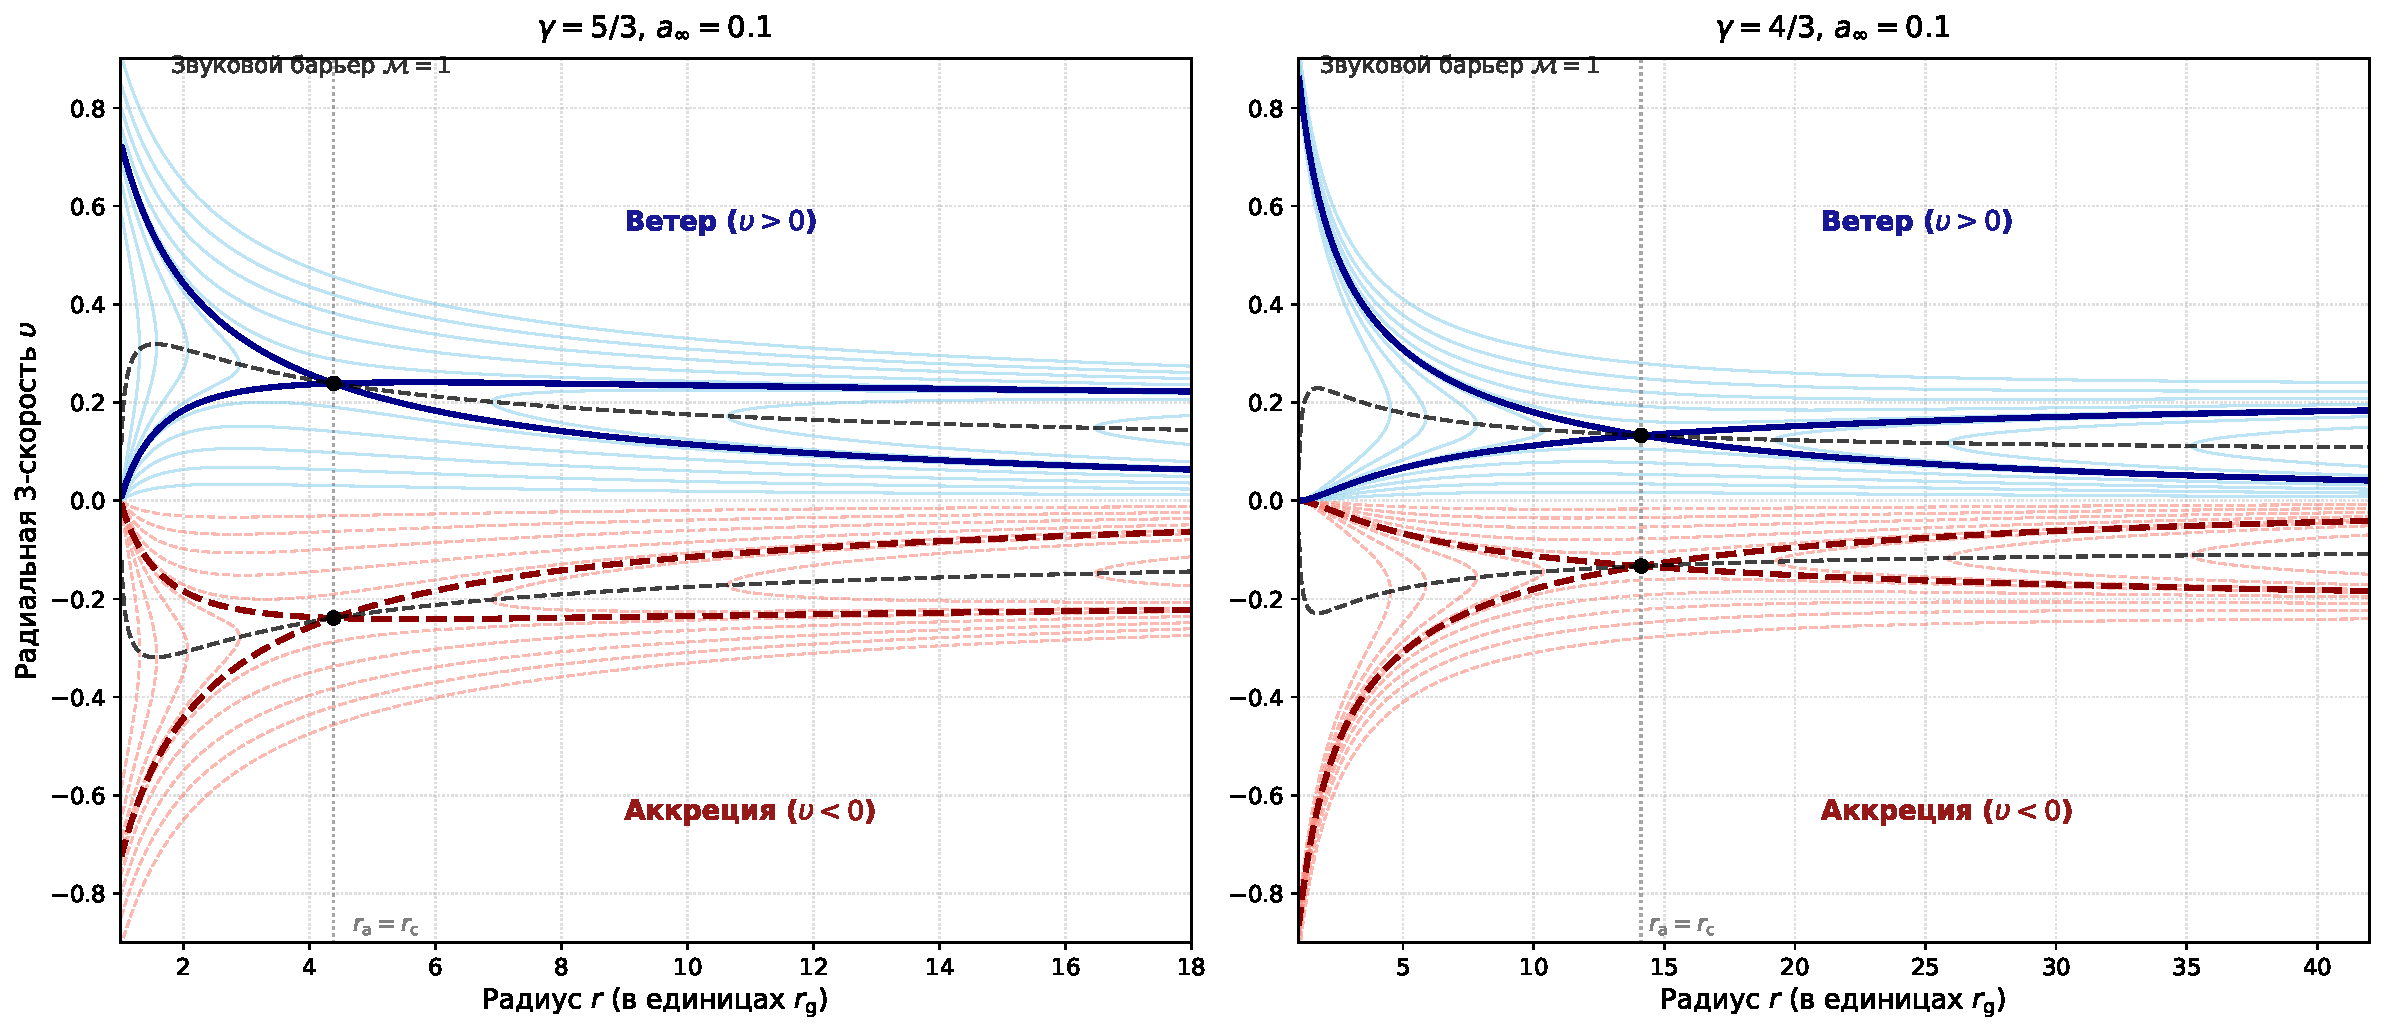
\includegraphics[width=\linewidth]{fig_phase_topology.pdf}
                % \fbox{\parbox{0.85\linewidth}{\centering\vspace{2cm}\textbf{[РИСУНОК 1]}\\[6pt] Топология стационарных решений потока Мишеля.\vspace{2cm}}}
                \caption{Топология стационарных решений в плоскости $(r, \mathcal{M})$, где $\mathcal{M}$ --- физическое число Маха, измеряемое локально статическим наблюдателем. При фиксированном интеграле Бернулли каждое решение является линией уровня потока барионов $\mathcal{J}$. Критическому потоку соответствует единственная трансзвуковая пара ветвей (аккреционная, $\upsilon < 0$, и ветровая, $\upsilon > 0$), пересекающихся в седловой звуковой точке $r = r_{\mathrm{c}}$. Горизонтальные сплошные черные линии отмечают звуковой барьер $|\mathcal{M}| = 1$, совпадающий с акустическим горизонтом $r = r_{\mathrm{a}}$.}
                \label{fig:phase-topology}
            \end{figure}
            
            Анализ опирается на следующие допущения: (i) стационарность и сферическая симметрия фона; (ii) модель совершенной жидкости с политропным уравнением состояния; (iii) отсутствие вращения и самогравитации аккрецирующего вещества; (iv) приближение геометрической оптики для линейных возмущений.

        \subsection{Две обращённые во времени ветви}\label{subsec:two-branches}
            Седловая структура критической точки~\eqref{eq:critical-point} подразумевает существование двух физически регулярных ветвей, имеющих одинаковые интегралы движения~\eqref{eq:michel-integrals} и одинаковое термодинамическое замыкание:
            \begin{itemize}
                \item \emph{Аккреционная ветвь}, $\upsilon < 0$, в которой поток ускоряется внутрь от состояния покоя на бесконечности, пересекает звуковой барьер при $r = r_{\mathrm{c}}$ и становится сверхзвуковым внутри акустического горизонта. Эта ветвь составляет классический поток Мишеля и порождает акустическую чёрную дыру.
                \item \emph{Ветровая ветвь}, $\upsilon > 0$, в которой поток выходит сверхзвуковым из акустического горизонта, замедляется наружу, проходя через звуковую точку, и приходит в состояние покоя на бесконечности. Эта ветвь является точным обращением аккреционной ветви во времени и порождает акустическую белую дыру.
            \end{itemize}
            Обе ветви удовлетворяют одному и тому же условию акустического горизонта $\eta^{rr}(r_{\mathrm{a}}) = 0$, причём $r_{\mathrm{a}} = r_{\mathrm{c}}$, и обе обладают одинаковой поверхностной гравитацией $\kappa$ и одинаковой формальной площадью акустического горизонта $\mathcal{A}_{\mathrm{a}}$~\cite{SemyannikovAV_AcousticGeometryAndSoundRayDynamicsInRelativisticSphericalAccretion_2026}. Два состояния, таким образом, термодинамически вырождены в кинематическом смысле, однако они разделены классически запрещённой областью.
            
            Классическая запрещённость перехода является прямым следствием законов сохранения. Поток барионов $\mathcal{J} = r^{2} n \upsilon$ должен оставаться постоянным вдоль любой классической траектории; непрерывный путь от аккреционной ветви ($\mathcal{J} < 0$) к ветровой ($\mathcal{J} > 0$) потребовал бы смены знака $\mathcal{J}$, что невозможно без нарушения закона сохранения барионов либо без прохождения через сингулярное состояние, где $n \to \infty$ или $\upsilon = 0$ всюду. Единственный регулярный путь, соединяющий две ветви, проходит через седловую точку, где $\upsilon = \upsilon_{\mathrm{c}} \neq 0$, но этот путь требует от потока бесконечно долго задерживаться в седле, что классически запрещено для стационарной конфигурации.
            
            Причинные структуры двух ветвей являются точными обращениями друг друга во времени~\cite{SemyannikovAV_GlobalAcousticGeometryOfMichelFlowInPainleveGullstrandCoordinates_2026}. Для аккреционной ветви исходящая акустическая характеристика замерзает на горизонте ($c_{+}|_{r_{\mathrm{a}}} = 0$), тогда как входящая остаётся конечной и отрицательной; для ветровой ветви роли двух характеристик меняются местами, и горизонт действует как односторонняя мембрана для входящих, а не исходящих возмущений. Эта замена является гидродинамическим аналогом дихотомии чёрной и белой дыр в вакуумной гравитации.

    \section{Формализм Пенлеве--Гульстранда для обеих ветвей}\label{sec:pg-framework}
        \subsection{Регулярное представление акустического ядра}\label{subsec:pg-core}
            Стандартные шварцшильдовские координаты сингулярны на гравитационном горизонте $r = 1$, что препятствует глобальному анализу причинной структуры. Следуя~\cite{SemyannikovAV_GlobalAcousticGeometryOfMichelFlowInPainleveGullstrandCoordinates_2026}, осуществляется переход к PG-базису, регулярному на обоих горизонтах. Замена временной координаты
            \begin{equation}
                v_{\mathrm{ff}}(r) \equiv -r^{-1/2}, \qquad \psi(r) \equiv -v_{\mathrm{ff}}\,f^{-1}, \qquad \mathrm{d}\check{t} = \mathrm{d}t + \psi(r)\,\mathrm{d}r,
                \label{eq:pg-transformation}
            \end{equation}
            приводит метрику~\eqref{eq:schwarzschild-metric} к регулярному виду $\check{g}_{\mu\nu}$:
            \begin{equation}
                \mathrm{d}s^{2} = -f\,\mathrm{d}\check{t}^{\,2} - 2\,v_{\mathrm{ff}}\,\mathrm{d}\check{t}\,\mathrm{d}r + \mathrm{d}r^{2} + r^{2}\,\mathrm{d}\theta^{2} + r^{2}\sin^{2}\!\theta\,\mathrm{d}\phi^{2}.
                \label{eq:pg-metric}
            \end{equation}
            В этих координатах сечения постоянного времени пространственноподобны и евклидовы, а свободное падение описывается регулярным сдвигом $v_{\mathrm{ff}} < 0$. 4-скорость потока в PG-базисе
            \begin{equation}
                \check{u}^{\mu} = \bigl(\check{\vartheta},\,\upsilon,\,0,\,0\bigr), \qquad \check{\vartheta} = \vartheta + \psi(r)\,\upsilon,
                \label{eq:four-velocity-pg}
            \end{equation}
            имеет конечный предел на гравитационном горизонте:
            \begin{equation}
                \check{\vartheta}\big|_{r=1} = \frac{1 + \upsilon_{\mathrm{g}}^{2}}{2\,|\upsilon_{\mathrm{g}}|} < \infty,
                \label{eq:vartheta-limit}
            \end{equation}
            где $\upsilon_{\mathrm{g}} \equiv \upsilon(1)$ --- радиальная скорость потока на гравитационном горизонте, что гарантирует регулярность $\check{\vartheta}$ на $r = 1$.
            
            Акустическое ядро в PG-базисе,
            \begin{equation}
                \zeta_{\mu\nu} = \check{g}_{\mu\nu} - \beta\,\check{u}_{\mu}\,\check{u}_{\nu}, \qquad \beta = a^{2} - 1,
                \label{eq:acoustic-core-pg}
            \end{equation}
            удовлетворяет тождеству для определителя
            \begin{equation}
                \zeta_{\check{t}\check{t}}\,\zeta_{rr} - \zeta_{\check{t}r}^{\,2} = -a^{2},
                \label{eq:determinant-identity}
            \end{equation}
            для любого $a > 0$, что отражает гиперболичность акустического ядра и исключает координатные вырождения. Условие акустического горизонта эквивалентно $\zeta_{\check{t}\check{t}} = 0$ и сводится к~\cite{SemyannikovAV_GlobalAcousticGeometryOfMichelFlowInPainleveGullstrandCoordinates_2026}
            \begin{equation}
                \beta(r_{\mathrm{a}})\,f(r_{\mathrm{a}})\,\vartheta^{2}(r_{\mathrm{a}}) = -1.
                \label{eq:horizon-condition-pg}
            \end{equation}
            Физически это означает, что формирование акустического горизонта определяется исключительно локальным числом Маха и не зависит от выбора временн\'{о}й координаты. PG-представление регулярно для обеих ветвей, поскольку преобразование~\eqref{eq:pg-transformation} зависит только от фоновой метрики Шварцшильда, а не от знака скорости жидкости.

        \subsection{Характеристические скорости для обеих ветвей}\label{subsec:characteristics-both}
            Характеристические скорости для радиальных лучей,
            \begin{equation}
                c_{\pm} = \frac{-\zeta_{\check{t}r} \pm a}{\zeta_{rr}},
                \label{eq:characteristic-speeds}
            \end{equation}
            конечны на обоих горизонтах~\cite{SemyannikovAV_GlobalAcousticGeometryOfMichelFlowInPainleveGullstrandCoordinates_2026}. Для \emph{аккреционной ветви} ($\upsilon < 0$) условие~\eqref{eq:horizon-condition-pg} даёт:
            \begin{equation}
                c_{+}\big|_{r_{\mathrm{a}}} = 0, \qquad c_{-}\big|_{r_{\mathrm{a}}} < 0,
                \label{eq:acc-characteristics}
            \end{equation}
            что означает формирование односторонней акустической мембраны: исходящие возмущения не могут покинуть сверхзвуковую область. Для \emph{ветровой ветви} ($\upsilon > 0$) роли двух характеристик меняются местами:
            \begin{equation}
                c_{-}\big|_{r_{\mathrm{a}}} = 0, \qquad c_{+}\big|_{r_{\mathrm{a}}} > 0,
                \label{eq:wind-characteristics}
            \end{equation}
            что означает, что горизонт действует как односторонняя мембрана для входящих, а не исходящих возмущений. Это определяющее свойство акустической белой дыры: возмущения могут выходить из горизонта, но не могут в него возвращаться. На гравитационном горизонте $r_{\mathrm{g}}$ обе характеристики конечны и отрицательны для обеих ветвей, и гравитационный горизонт не является акустическим~\cite{SemyannikovAV_GlobalAcousticGeometryOfMichelFlowInPainleveGullstrandCoordinates_2026}.
            
            Два набора характеристик~\eqref{eq:acc-characteristics} и~\eqref{eq:wind-characteristics} являются точными обращениями друг друга во времени и имеют одинаковую поверхностную гравитацию и одинаковую формальную площадь акустического горизонта~\cite{SemyannikovAV_AcousticGeometryAndSoundRayDynamicsInRelativisticSphericalAccretion_2026}.

    \section{Переход между вырожденными ветвями: однопараметрическая модель}\label{sec:transition-model}
        \subsection{Энергетический функционал и вырождение ветвей}\label{subsec:energy-functional}
            Полная энергия конфигурации жидкости на фоне Шварцшильда, измеряемая стационарным наблюдателем на бесконечности, определяется интегралом от $(-T^{t}_{t})$ по объёму:
            \begin{equation}
                E[\upsilon, n] = \int_{1}^{r_{\mathrm{B}}} 4\pi r^{2}\left[(\varepsilon + p)(f + \upsilon^{2}) - p\right]\,\mathrm{d}r,
                \label{eq:energy-functional}
            \end{equation}
            где $r_{\mathrm{B}} \sim a_{\infty}^{-2}$ --- радиус Бонди, служащий естественным внешним обрезателем сферической аккреции, $\varepsilon$ --- полная плотность энергии, $p$ --- давление.

            Функционал~\eqref{eq:energy-functional} представляет собой модельную энергию конфигурации, построенную интегрированием проекции $T^{\hat{t}}_{\hat{t}}$ тензора энергии-импульса жидкости в локально статической системе отсчёта $(\hat{t}, \hat{r}, \hat{\theta}, \hat{\phi})$ по координатному объёму $4\pi r^{2}\,\mathrm{d}r$. Это отличается от точной сохраняющейся энергии, требующей интегрирования по собственному объёму (с метрическим фактором $f^{-1/2} \approx 1 + 1/(2r)$), на член порядка $p/r$, несущественный в дозвуковой области за исключением непосредственной окрестности $r_{\mathrm{c}}$, где поправка не превышает нескольких процентов; для холодных потоков ($r_{\mathrm{c}} \gg 1$) поправка пренебрежимо мала всюду. Точный вид сохраняющейся энергии в метрике Шварцшильда включает дополнительные метрические факторы, которые, однако, не изменяют топологию экстремумов при $q = \pm 1$ и не влияют на структуру инстантонного действия. Сверхзвуковая оболочка $1 < r < r_{\mathrm{c}}$ исключена из эффективного момента инерции, вводимого в разд.~\ref{subsec:collective-coordinate}, поскольку она причинно отсоединена от внешней области.

            Скорость $\upsilon$ входит в~\eqref{eq:energy-functional} квадратично, поэтому аккреционная ветвь ($\upsilon < 0$) и ветровая ветвь ($\upsilon > 0$) обладают тождественной энергией:
            \begin{equation}
                E[\upsilon_{\mathrm{acc}}, n] = E[-\upsilon_{\mathrm{acc}}, n].
                \label{eq:energy-degeneracy}
            \end{equation}
            Два стационарных решения являются стационарными точками (экстремумами при соответствующих гидродинамических ограничениях) одного и того же функционала~\eqref{eq:energy-functional}.
            
            Барьер между двумя ветвями не является \emph{термодинамическим фазовым барьером}: разность свободных энергий двух состояний тождественно равна нулю, $\Delta F = 0$, и ни одна из ветвей не является метастабильной относительно другой. Вместе с тем в пространстве коллективной координаты $q$ состояния $\pm 1$ разделены \emph{макроскопическим инерционно-кинематическим барьером}: для перевода конфигурации из одной ветви в другую необходимо совершить работу против градиентов давления и гравитационного поля, чтобы остановить макроскопический поток и развернуть его в противоположном направлении. Этот барьер имеет чисто механическую природу и возникает из инерции конечной массы жидкости, а не из термодинамической неравноценности двух фаз.

        \subsection{Коллективная координата и эффективный лагранжиан}\label{subsec:collective-coordinate}
            Для описания перехода вводится безразмерная коллективная координата $q(\tau) \in [-1, +1]$, параметризующая степень обращения потока, где $\tau$ --- евклидово время:
            \begin{equation}
                \upsilon(r, q) = q \cdot \upsilon_{\mathrm{acc}}(r), \qquad q = -1: \text{аккреция}, \quad q = 0: \text{остановленный поток}, \quad q = +1: \text{ветер}.
                \label{eq:collective-coordinate}
            \end{equation}
            Введение $q$ и учёт перестройки профиля $n(r, q)$ при сохранении полного числа барионов приводит к модельному эффективному лагранжиану:
            \begin{equation}
                L_{\mathrm{eff}} = \frac{1}{2}\,I\,\dot{q}^{\,2} - V(q),
                \label{eq:effective-lagrangian}
            \end{equation}
            где эффективный момент инерции потока
            \begin{equation}
                I = \int_{r_{\mathrm{c}}}^{r_{\mathrm{B}}} 4\pi r^{2}\,\rho\,\upsilon_{\mathrm{acc}}^{2}\,\mathrm{d}r, \qquad \rho \equiv \varepsilon + p,
                \label{eq:effective-inertia}
            \end{equation}
            а $V(q)$ --- модельный эффективный потенциал, удовлетворяющий условиям $V(\pm 1) = 0$ и $V(0) = \Delta E > 0$. Область $r < r_{\mathrm{c}}$ исключена из~\eqref{eq:effective-inertia}, поскольку акустический горизонт $r = r_{\mathrm{c}}$ является регулярной особой точкой линеаризованных уравнений Эйлера~\cite{SemyannikovAV_PerturbationSpectrumOfMichelFlowAcousticVorticalAndEntropyModes_2026}, а сверхзвуковая оболочка причинно отсоединена от внешней области; это разделение остаётся корректным и в евклидовом секторе после поворота Вика.
            
            Сходимость интеграла~\eqref{eq:effective-inertia} проверяется явно. Из закона сохранения барионов $r^{2}n|\upsilon| = |\mathcal{J}|$ следует $\rho\,\upsilon^{2} = h|\mathcal{J}|\,|\upsilon|/r^{2}$, откуда подынтегральное выражение $4\pi r^{2}\rho\,\upsilon^{2} = 4\pi|\mathcal{J}|\,h\,|\upsilon|$. На бесконечности $|\upsilon| \sim r^{-2}$ и $h \to h_{\infty}$, поэтому подынтегральное выражение убывает как $r^{-2}$, и интеграл сходится. Вблизи $r_{\mathrm{c}}$ все величины конечны, и подынтегральное выражение не имеет особенностей. Значительная часть вклада возникает из окрестности акустического горизонта, где $|\upsilon| \sim a_{\mathrm{c}}$ и плотность энтальпии усилена сжатием потока (рис.~\ref{fig:inertia-localization}).
            
            \begin{figure}[htb]
                \centering
                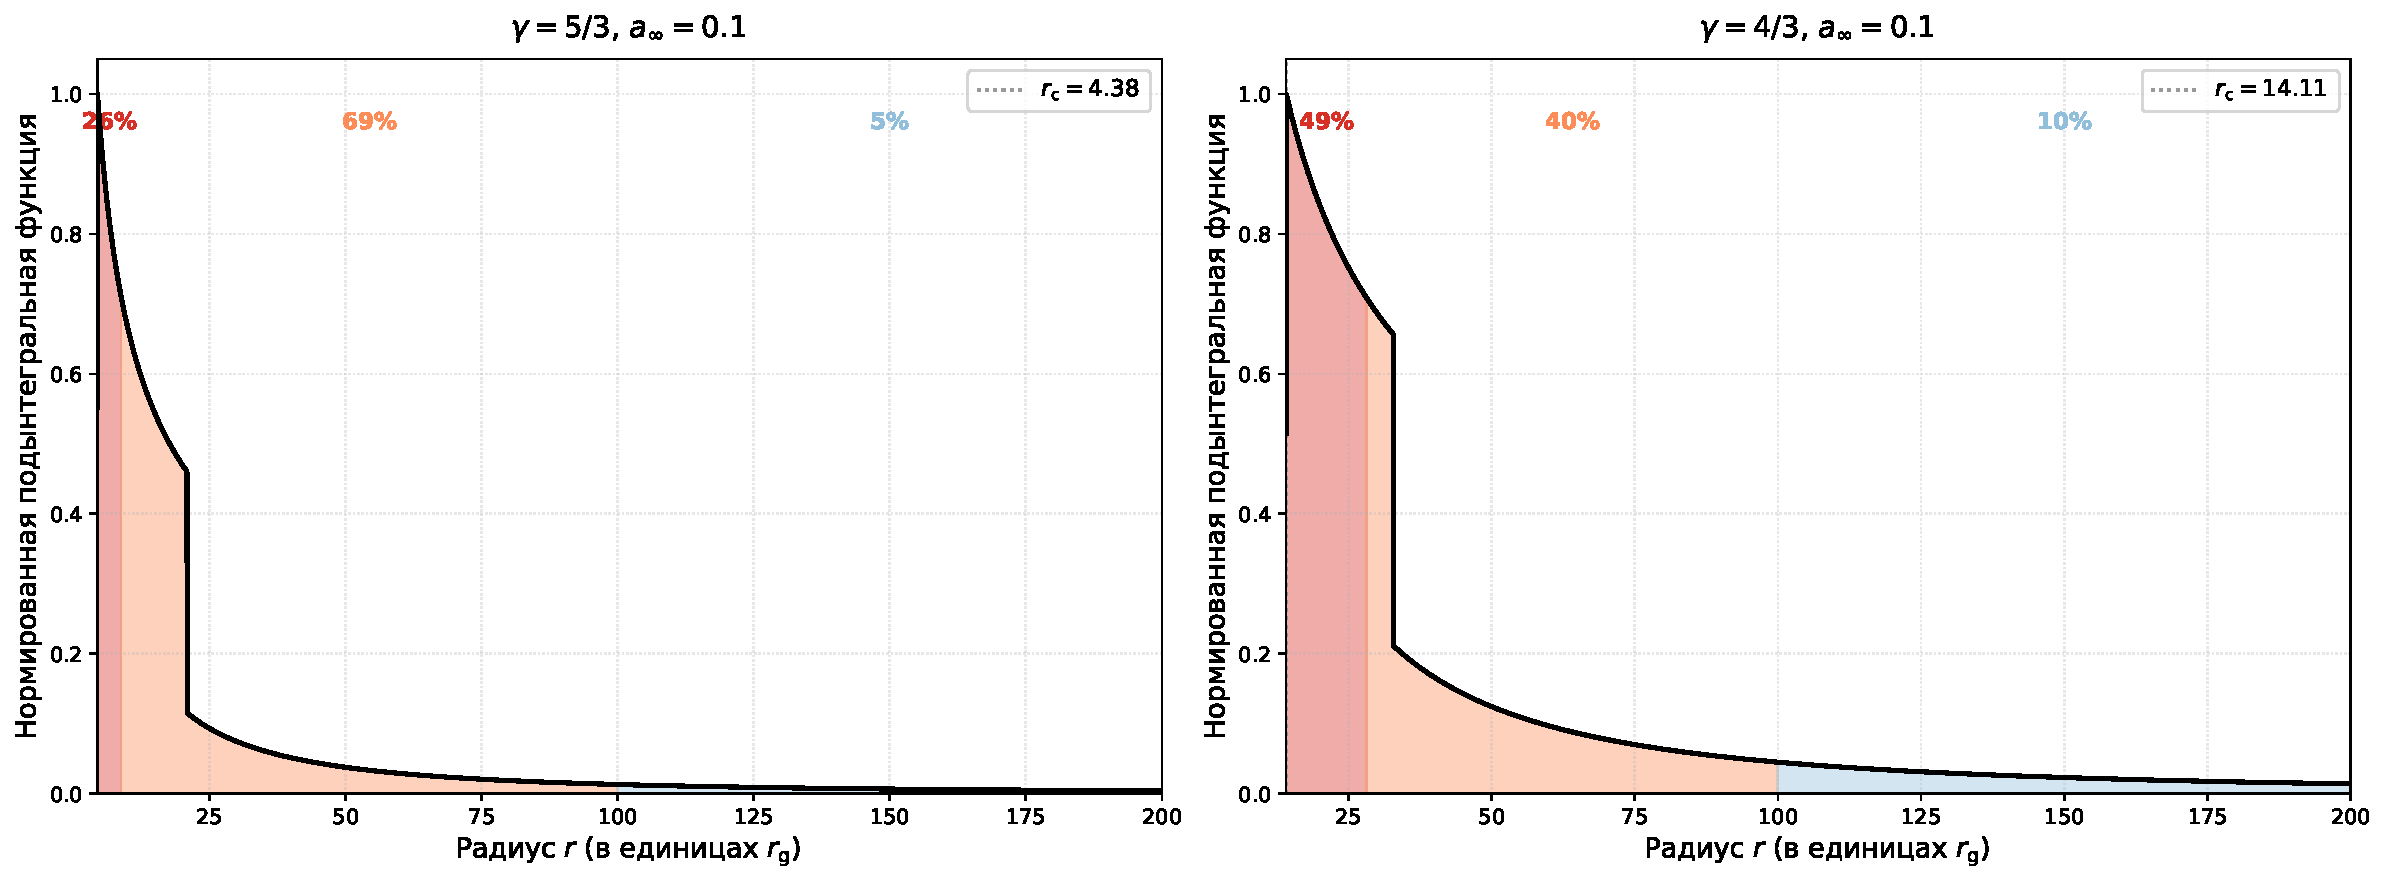
\includegraphics[width=\linewidth]{fig_inertia_localization.pdf}
                \caption{Подынтегральная функция $4\pi r^{2}\rho\,\upsilon_{\mathrm{acc}}^{2}(r)$ из~\eqref{eq:effective-inertia}, нормированная на своё максимальное значение, как функция $r$ (в единицах $r_{\mathrm{g}}$) при $a_{\infty} = 0{,}1$. Левая панель: $\gamma = 5/3$; правая панель: $\gamma = 4/3$. Закрашенные области выделяют вклады трёх радиальных интервалов: $[r_{\mathrm{c}}, 2r_{\mathrm{a}}]$ (область акустического горизонта), $[2r_{\mathrm{a}}, r_{\mathrm{B}}/2]$ (промежуточная зона) и $[r_{\mathrm{B}}/2, r_{\mathrm{B}}]$ (внешняя зона). Вертикальная штриховая линия отмечает $r_{\mathrm{c}}$. Численные доли вклада каждого интервала в полный момент инерции $I$ указаны на вставках.}
                \label{fig:inertia-localization}
            \end{figure}

        \subsection{Природа энергетического барьера}\label{subsec:barrier-origin}
            Эффективный потенциал $V(q)$ имеет максимум при $q = 0$.
            
            Прямая подстановка $\upsilon(r, q) = q \cdot \upsilon_{\mathrm{acc}}(r)$ в~\eqref{eq:energy-functional} при \emph{фиксированном} профиле $n(r) = n_{\mathrm{acc}}(r)$ даёт квадратичную зависимость $E(q) = E(0) + I q^{2}/2$, которая имеет минимум при $q = 0$, а не двойную яму с максимумами при $q = \pm 1$. Для получения потенциала с двумя минимумами необходимо учесть перестройку профиля $n(r, q)$ при изменении $q$, что требует решения полной задачи гидростатического равновесия с учётом сохранения барионов и условия Бернулли~\eqref{eq:michel-integrals} для каждого значения $q$.
            
            В простейшей симметричной феноменологической модели принимается потенциал двойной ямы:
            \begin{equation}
                V(q) = \Delta E\,(1 - q^{2})^{2},
                \label{eq:double-well-potential}
            \end{equation}
            что обеспечивает минимумы при $q = \pm 1$ и максимум $V(0) = \Delta E$ при $q = 0$ (рис.~\ref{fig:double-well-potential}).
            
            \begin{figure}[htb]
                \centering
                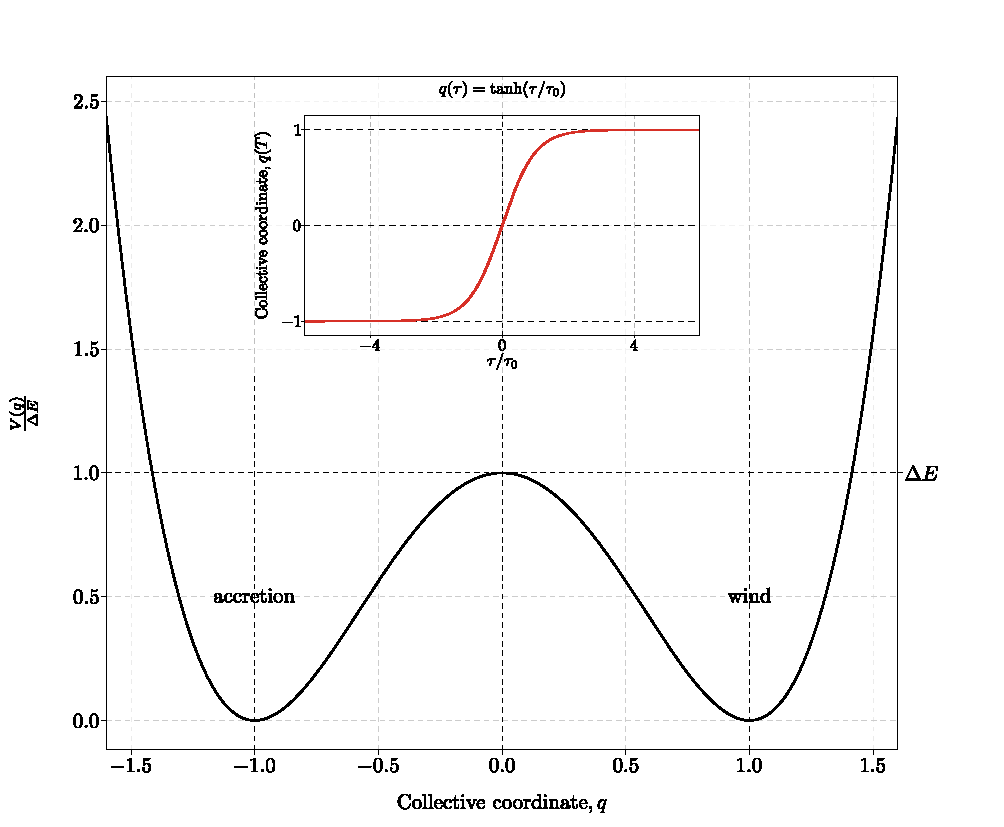
\includegraphics[width=\linewidth]{fig_double_well_potential.pdf}
                % \fbox{\parbox{0.67\linewidth}{\centering\vspace{2cm}\textbf{[РИСУНОК 3]}\\[6pt] Модельный потенциал двойной ямы и инстантонная траектория.\vspace{2cm}}}
                \caption{Модельный потенциал двойной ямы $V(q) = \Delta E(1-q^{2})^{2}$ из~\eqref{eq:double-well-potential} (сплошная чёрная кривая); потенциал $V$ дан в единицах $\Delta E$, коллективная координата $q$ безразмерна. Минимумы при $q = \pm 1$ соответствуют аккреционной и ветровой ветвям; максимум $V(0) = \Delta E$ при $q = 0$ --- остановленному потоку. Пунктирная горизонтальная линия отмечает уровень $\Delta E$. Вставка: инстантонная траектория $q(\tau) = \tanh(\tau/\tau_{0})$ как функция евклидова времени $\tau$ в единицах $\tau_{0}$.}
                \label{fig:double-well-potential}
            \end{figure}
            
            При $q = 0$ кинетическая энергия макроскопического потока обращается в нуль, однако профиль плотности $n(r)$ и энтальпии $h(r)$, соответствующий стационарному течению, не может мгновенно релаксировать к новому гидростатическому равновесию, определяемому условием $\nabla p = -(\varepsilon + p)\,\nabla\Phi_{\mathrm{eff}}$, где $\Phi_{\mathrm{eff}}$ --- эффективный гравитационный потенциал (в ньютоновском пределе $\Phi_{\mathrm{eff}} = -1/(2r)$). В гравитационном поле Шварцшильда гидростатический профиль энтальпии не является однородным: он нарастает к центру, компенсируя гравитационное притяжение. Одновременно полное число барионов в дозвуковой области сохраняется, что накладывает интегральное ограничение на допустимые профили $n(r)$. Именно рассогласование между инерционно замороженным профилем плотности и отсутствием макроскопической скорости создаёт избыточную энергию $\Delta E$, которая представляет собой минимальную энергетическую стоимость нарушения релятивистского интеграла Бернулли~\eqref{eq:michel-integrals} при остановке потока.
            
            Высота барьера оценивается как энергия, необходимая для остановки потока, и масштабируется как $\Delta E \approx \alpha\, I \upsilon_{\mathrm{c}}^{2}$, где $\upsilon_{\mathrm{c}}$ --- скорость потока в звуковой точке, а безразмерный коэффициент $\alpha \sim 0{,}3$--$0{,}9$ зависит от пары $(\gamma, a_{\infty})$: для $a_{\infty} = 0{,}1$ коэффициент составляет $\alpha \approx 0{,}31$ при $\gamma = 5/3$ и $\alpha \approx 0{,}52$ при $\gamma = 4/3$; при $a_{\infty} = 0{,}05$ коэффициент может достигать $\alpha \approx 0{,}92$ для $\gamma = 4/3$ и снижаться до $\alpha \approx 0{,}27$ для $\gamma = 5/3$, что отражает усиление зависимости от уравнения состояния в холодном пределе.

        \subsection{Инстантонное действие}\label{subsec:instanton-action}
            Евклидов поворот $\tau = it$ преобразует~\eqref{eq:effective-lagrangian} в евклидов лагранжиан:
            \begin{equation}
                L_{\mathrm{E}} = \frac{1}{2}\,I\,\dot{q}^{\,2} + V(q).
                \label{eq:euclidean-lagrangian}
            \end{equation}
            Инстантонная траектория $q(\tau)$ соединяет $q(-\infty) = -1$ с $q(+\infty) = +1$ и удовлетворяет евклидову уравнению движения:
            \begin{equation}
                I\,\ddot{q} = \frac{\mathrm{d}V}{\mathrm{d}q} = -4\Delta E\,q\,(1 - q^{2}).
                \label{eq:euclidean-eom}
            \end{equation}
            Для потенциала~\eqref{eq:double-well-potential} решение имеет вид:
            \begin{equation}
                q(\tau) = \tanh\left(\frac{\tau}{\tau_{0}}\right), \qquad \tau_{0} = \sqrt{\frac{I}{2\,\Delta E}}.
                \label{eq:instanton-solution}
            \end{equation}
            Инстантонное действие вычисляется интегрированием~\eqref{eq:euclidean-lagrangian} вдоль~\eqref{eq:instanton-solution}:
            \begin{equation}
                \mathcal{S}_{\mathrm{inst}} = \int_{-\infty}^{+\infty} L_{\mathrm{E}}\,\mathrm{d}\tau = \int_{-1}^{+1}\sqrt{2\,I\,V(q)}\,\mathrm{d}q = \sqrt{2\,I\,\Delta E} \int_{-1}^{+1} (1 - q^{2})\,\mathrm{d}q.
                \label{eq:instanton-action-integral}
            \end{equation}
            Поскольку элементарное интегрирование даёт
            \begin{equation}
                \int_{-1}^{+1} (1 - q^{2})\,\mathrm{d}q = \left[ q - \frac{q^{3}}{3} \right]_{-1}^{+1} = \frac{4}{3},
                \label{eq:q-integral}
            \end{equation}
            инстантонное действие принимает конечно определённый вид:
            \begin{equation}
                \mathcal{S}_{\mathrm{inst}} = \frac{4}{3}\sqrt{2\,I\,\Delta E}.
                \label{eq:instanton-action-final}
            \end{equation}
            Это выражение является конечно определённым: оба множителя $I$ и $\Delta E$ конечны, и действие не содержит расходимостей. Формула~\eqref{eq:instanton-action-final} специфична для симметричного потенциала~\eqref{eq:double-well-potential}; для общего (не обязательно симметричного) потенциала $V(q)$ инстантонное действие даётся интегралом $\mathcal{S}_{\mathrm{inst}} = \int_{-1}^{+1}\sqrt{2\,I\,V(q)}\,\mathrm{d}q$.

        \subsection{Вероятность туннелирования и эффективная постоянная Планка}\label{subsec:tunneling-probability}
            Вероятность перехода в единицу времени даётся полуклассической формулой:
            \begin{equation}
                \Gamma \sim \omega_{0}\,\exp\left(-\frac{\mathcal{S}_{\mathrm{inst}}}{\hbar_{\mathrm{eff}}}\right),
                \label{eq:tunneling-rate-final}
            \end{equation}
            где $\omega_{0} = \sqrt{V''(1)/I} = \sqrt{8\Delta E/I}$ --- частота малых осцилляций вблизи минимума, а $\hbar_{\mathrm{eff}}$ --- эффективная постоянная Планка системы.
            
            Связь инстантонного действия с инвариантами акустического горизонта устанавливается через формальную площадь и поверхностную гравитацию, табулированные в~\cite{SemyannikovAV_AcousticGeometryAndSoundRayDynamicsInRelativisticSphericalAccretion_2026}.
            
            Для классической идеальной жидкости $\hbar_{\mathrm{eff}} \to 0$, и вероятность туннелирования тождественно равна нулю. Формула~\eqref{eq:tunneling-rate-final} приобретает физический смысл только для систем с квантовой микроструктурой. Параметр $\hbar_{\mathrm{eff}}$ представляет собой отношение микроскопического масштаба (например, длины Комптона частицы $\lambda_{\mathrm{C}} = \hbar/(m c_{\mathrm{s}})$ или длины когерентности в конденсате Бозе--Эйнштейна) к макроскопическому радиусу $r_{\mathrm{g}}$. Для астрофизической плазмы ($m \sim m_{p}$, $r_{\mathrm{g}} \sim 10^{13}$ см) параметр $\hbar_{\mathrm{eff}} \sim 10^{-41}$, и туннелирование строго нереализуемо. Для лабораторных аналогов (конденсаты Бозе--Эйнштейна, сверхтекучий гелий) $\hbar_{\mathrm{eff}}$ может достигать $10^{-2}$--$10^{-4}$; однако даже при $\hbar_{\mathrm{eff}} \sim 10^{-2}$ и $\mathcal{S}_{\mathrm{inst}} \sim 30$ экспонента $\exp(-\mathcal{S}_{\mathrm{inst}}/\hbar_{\mathrm{eff}}) \sim \exp(-3000)$ исчезающе мала. Туннелирование \emph{всей} макроскопической конфигурации практически ненаблюдаемо ни в астрофизических, ни в лабораторных условиях; физический интерес настоящего результата является преимущественно концептуальным и состоит в установлении структурной аналогии с вакуумными переходами чёрная дыра -- белая дыра~\cite{VolovikGE_PainleveGullstrandCoordinatesForSchwarzschildDeSitterSpacetime_2023}.

    \section{Обсуждение}\label{sec:discussion}
        \subsection{Аналогия с персистентным током}\label{subsec:persistent-current}
            Структура задачи~\eqref{eq:effective-lagrangian}--\eqref{eq:instanton-action-final} идентична обращению персистентного тока в сверхпроводящем кольце или СКВИД-контуре. Соответствие между двумя системами представлено в табл.~\ref{tab:analogy}.
            \begin{table}[htb]
                \centering
                \caption{Аналогия между потоком Мишеля и персистентным током в сверхпроводящем кольце.}
                \label{tab:analogy}
                \small
                \begin{tabular}{lll}
                    \toprule
                    & Персистентный ток & Поток Мишеля \\
                    \midrule
                    Вырожденные состояния & $\pm J$ & $\upsilon < 0$ и $\upsilon > 0$ \\
                    Барьер & Индуктивность $LJ^{2}/2$ & Инерция потока $I$ \\
                    Коллективная координата & Фаза параметра порядка $\phi$ & Степень обращения $q$ \\
                    Инстантон & Фазовый сдвиг на $2\pi$ (квантование циркуляции) & Обращение $\upsilon(r)$ \\
                    Подавление & $\exp(-S_{\mathrm{SQUID}}/\hbar)$ & $\exp(-\mathcal{S}_{\mathrm{inst}}/\hbar_{\mathrm{eff}})$ \\
                    Квант действия & $\hbar$ & $\hbar_{\mathrm{eff}}$ \\
                    \bottomrule
                \end{tabular}
            \end{table}
            В сверхпроводящем кольце с джозефсоновским контактом евклидов лагранжиан имеет вид $L_{\mathrm{E}} = \frac{1}{2}L\dot{\phi}^{2} + E_{J}(1 - \cos\phi)$, где $L$ --- индуктивность, $E_{J}$ --- энергия джозефсоновской связи. При $E_{J} \ll LJ^{2}/2$ инстантонное действие принимает вид $\mathcal{S}_{\mathrm{inst}} \approx \frac{4}{3}\sqrt{2LJ^{2}E_{J}}$, что структурно идентично формуле~\eqref{eq:instanton-action-final} с заменой $L \to I$, $E_{J} \to \Delta E$. Это соответствие показывает, что формула~\eqref{eq:instanton-action-final} не является ad hoc конструкцией, а имеет точный аналог в хорошо изученной квантовой системе.
            
            Ключевое отличие состоит в том, что в сверхпроводящем кольце барьер создаётся джозефсоновской связью, тогда как в потоке Мишеля барьер обусловлен нарушением интеграла Бернулли при остановке потока. В обоих случаях подавление определяется макроскопической инерцией системы.

        \subsection{Глобальное туннелирование и нуклеация}\label{subsec:nucleation}
            Для бесконечной системы одновременный переворот всей конфигурации имеет нулевую вероятность. Физически реализуемый механизм в квантовой теории поля --- нуклеация пузыря новой фазы~\cite{ColemanS_AspectsOfSymmetry_1985}:
            \begin{equation}
                S_{\mathrm{bubble}}(R) = 4\pi R^{2}\sigma - \frac{4\pi}{3}R^{3}\Delta\mathcal{E},
                \label{eq:coleman-action}
            \end{equation}
            где $\sigma$ --- поверхностное натяжение стенки, $\Delta\mathcal{E}$ --- разность плотностей энергии двух фаз. Для потока Мишеля стандартная нуклеация неприменима по двум причинам. Во-первых, $\Delta\mathcal{E} = 0$ (ветви вырождены), и экстремум~\eqref{eq:coleman-action} по $R$ не существует: критический радиус пузыря $R_{\mathrm{c}} = 2\sigma/\Delta\mathcal{E}$ расходится, а действие нуклеации $S_{\mathrm{bubble}} \to \infty$. Во-вторых, ветровая ветвь неустойчива: зародыш ветровой конфигурации немедленно разрушается из-за бесконечного синего смещения на горизонте белой дыры~\cite{SemyannikovAV_GlobalAcousticGeometryOfMichelFlowInPainleveGullstrandCoordinates_2026}.
            
            Глобальное туннелирование~\eqref{eq:tunneling-rate-final} является корректной постановкой для конечной системы радиуса $r_{\mathrm{B}}$. Радиус Бонди служит естественным обрезателем, делающим задачу конечномерной. Вероятность~\eqref{eq:tunneling-rate-final} конечна, но экспоненциально подавлена фактором $\exp(-\mathcal{S}_{\mathrm{inst}}/\hbar_{\mathrm{eff}})$.

        \subsection{Предэкспоненциальный множитель и отрицательная мода}\label{subsec:prefactor}
            Предэкспоненциальный множитель $\omega_{0}$ в~\eqref{eq:tunneling-rate-final} формально определяется отношением функциональных определителей флуктуаций вокруг инстантона и вокруг вакуума~\cite{ColemanS_AspectsOfSymmetry_1985}:
            \begin{equation}
                \omega_{0} \sim \left|\frac{\det'\bigl[-\partial_{\tau}^{2} + V''(q_{\mathrm{inst}})\bigr]}{\det\bigl[-\partial_{\tau}^{2} + V''(q_{\mathrm{vac}})\bigr]}\right|^{-1/2},
                \label{eq:prefactor-determinant}
            \end{equation}
            где штрих при $\det'$ означает исключение нулевых мод и отрицательной моды инстантона. В определитель входят вклады всех трёх семейств возмущений потока Мишеля --- акустических, вихревых и энтропийных мод~\cite{SemyannikovAV_PerturbationSpectrumOfMichelFlowAcousticVorticalAndEntropyModes_2026}.
            
            Физический смысл исключённых мод является стандартным~\cite{ColemanS_AspectsOfSymmetry_1985}. Нулевая мода соответствует трансляционной инвариантности инстантона во времени: сдвиг $\tau \to \tau + \tau_{0}$ не изменяет действия и порождает непрерывное семейство эквивалентных траекторий. Отрицательная мода (мнимая частота) соответствует неустойчивости седловой точки $q = 0$ и отвечает за сам факт распада: наличие ровно одной отрицательной моды является необходимым условием применимости формулы Колмана для скорости распада и обеспечивает конечность и положительность вероятности туннелирования.

        \subsection{Связь с поверхностной гравитацией и квазинормальными модами}\label{subsec:kappa-connection}
            Поверхностная гравитация $\kappa$, вычисленная в работе~\cite{SemyannikovAV_AcousticGeometryAndSoundRayDynamicsInRelativisticSphericalAccretion_2026}, определяет характерный временной масштаб рингдауна: $\tau_{\mathrm{QNM}} \sim \kappa^{-1}$. Длительность инстантона~\eqref{eq:instanton-solution} составляет $\tau_{0} = \sqrt{I/(2\Delta E)}$.
            
            Из табл.~\ref{tab:instanton-parameters} и значений $\kappa$, табулированных в~\cite{SemyannikovAV_AcousticGeometryAndSoundRayDynamicsInRelativisticSphericalAccretion_2026}, следует, что $\tau_{0}^{-1} \gg \kappa$ для всех рассматриваемых параметров: отношение $\tau_{0}^{-1}/\kappa$ составляет от $\sim 14$ ($\gamma = 5/3$, $a_{\infty} = 0{,}1$) до $\sim 200$ ($\gamma = 4/3$, $a_{\infty} = 0{,}05$).
            \begin{figure}[htb]
                \centering
                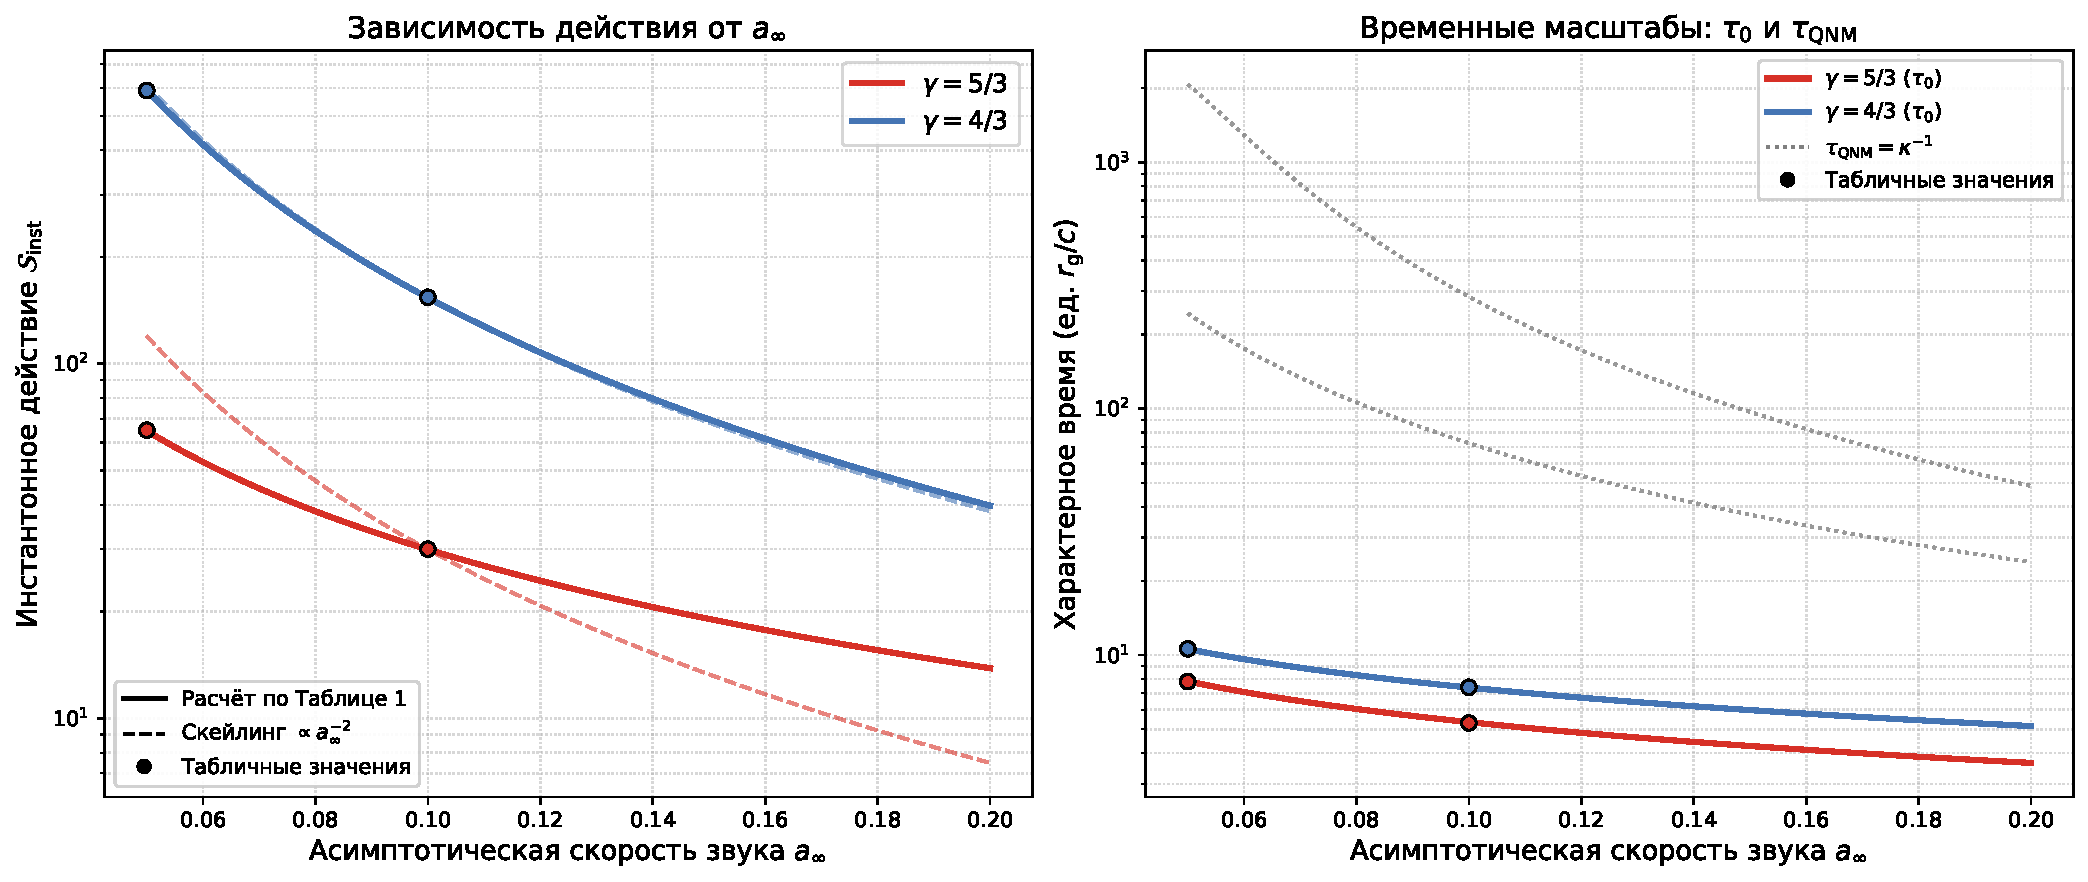
\includegraphics[width=0.88\linewidth]{fig_instanton_scaling.pdf}
                % \fbox{\parbox{0.85\linewidth}{\centering\vspace{2cm}\textbf{[РИСУНОК 4]}\\[6pt] Зависимость инстантонного действия и временных масштабов от $a_{\infty}$.\vspace{2cm}}}
                \caption{Зависимость инстантонного действия и характерных временных масштабов от асимптотической скорости звука $a_{\infty}$. Левая панель: инстантонное действие $\mathcal{S}_{\mathrm{inst}}$, вычисленное по формулам~\eqref{eq:instanton-action-final} и~\eqref{eq:instanton-solution} из значений $I$ и $\Delta E$ таблицы~\ref{tab:instanton-parameters} (сплошные кривые; маркеры --- табличные значения при $a_{\infty} = 0{,}05$ и $0{,}10$); штриховые кривые --- опорный скейлинг $\propto a_{\infty}^{-2}$, нормированный в точке $a_{\infty} = 0{,}1$. Правая панель: характерное время инстантона $\tau_{0} = \sqrt{I/(2\Delta E)}$ (сплошные кривые; маркеры --- табличные значения) и время рингдауна $\tau_{\mathrm{QNM}} = \kappa^{-1}$, где $\kappa$ взята из таблицы~2 сопутствующего исследования~\cite{SemyannikovAV_AcousticGeometryAndSoundRayDynamicsInRelativisticSphericalAccretion_2026}. Во всём исследованном диапазоне $\tau_{0} \ll \tau_{\mathrm{QNM}}$, что подтверждает разделение масштабов $\tau_{0}^{-1} \gg \kappa$.}
                \label{fig:instanton-scaling}
            \end{figure}
            Это означает, что инстантон длится значительно меньше одного периода квазинормальной моды, и акустические моды являются \emph{замороженными} на масштабе времени инстантона (внезапное приближение).
            \begin{table}[htb]
                \centering
                \caption{Численные оценки параметров инстантона. Значения $r_{\mathrm{c}}$ и $a_{\mathrm{c}}$ взяты из~\cite{SemyannikovAV_AcousticGeometryAndSoundRayDynamicsInRelativisticSphericalAccretion_2026}; параметры $I$, $\Delta E$, $\mathcal{S}_{\mathrm{inst}}$ и $\tau_{0}$ вычислены по формулам~\eqref{eq:effective-inertia}, \eqref{eq:double-well-potential}, \eqref{eq:instanton-action-final} и~\eqref{eq:instanton-solution}.}
                \label{tab:instanton-parameters}
                \small
                \begin{tabular}{lcccccc}
                    \toprule
                    $\gamma$ & $a_{\infty}$ & $r_{\mathrm{c}}$ & $I$ & $\Delta E$ & $\mathcal{S}_{\mathrm{inst}}$ & $\tau_{0}$ \\
                    \midrule
                    $5/3$ & $0{,}05$ & $8{,}13$ & $3{,}8 \cdot 10^{2}$ & $3{,}1$ & $65$ & $7{,}8$ \\
                    $5/3$ & $0{,}10$ & $4{,}38$ & $1{,}2 \cdot 10^{2}$ & $2{,}1$ & $30$ & $5{,}3$ \\
                    \midrule
                    $4/3$ & $0{,}05$ & $51{,}67$ & $4{,}7 \cdot 10^{3}$ & $21$ & $590$ & $10{,}6$ \\
                    $4/3$ & $0{,}10$ & $14{,}11$ & $8{,}5 \cdot 10^{2}$ & $7{,}8$ & $154$ & $7{,}4$ \\
                    \bottomrule
                \end{tabular}
            \end{table}
            
            Для более холодного потока ($\gamma = 4/3$) акустический горизонт расположен дальше ($r_{\mathrm{c}} \approx 14{,}11$ против $4{,}38$ при $a_{\infty} = 0{,}1$), что приводит к большему моменту инерции и, соответственно, к большему инстантонному действию. Уменьшение $a_{\infty}$ от $0{,}1$ до $0{,}05$ увеличивает $r_{\mathrm{c}}$ и, следовательно, $\mathcal{S}_{\mathrm{inst}}$, что подтверждает рост подавления туннелирования в холодном пределе (рис.~\ref{fig:instanton-scaling}). Это означает, что туннелирование сильнее подавлено для более холодных потоков, что согласуется с физической интуицией: чем дальше горизонт, тем больше масса жидкости, которую необходимо остановить и развернуть.

        \subsection{Пределы применимости}\label{subsec:limitations}
            Настоящий анализ опирается на следующие ограничения.
            
            Во-первых, однопараметрическая редукция предполагает, что переход описывается единственной коллективной координатой $q$. Полная гидродинамическая задача содержит бесконечное число степеней свободы, и инстантонная траектория в полном конфигурационном пространстве может отличаться от~\eqref{eq:instanton-solution}. Формула~\eqref{eq:instanton-action-final} даёт оценку действия; точное значение требует решения полной евклидовой задачи. Критерий применимости редукции требует, чтобы все остальные моды были тяжёлыми по сравнению с модой $q$, то есть их характерные частоты должны удовлетворять условию $\omega_{n} \gg \tau_{0}^{-1}$. Для акустических мод это условие выполняется ($\tau_{0}^{-1} \gg \kappa$); однако для адвектируемых вихревых и энтропийных мод разделение масштабов становится менее выраженным: в протяжённой ньютоновской оболочке снаружи отступающего горизонта их характерные частоты малы, и для более холодных потоков ($a_{\infty} \lesssim 0{,}05$) формула~\eqref{eq:tunneling-rate-final} даёт оценочное значение.
            
            Во-вторых, эффективный потенциал~\eqref{eq:double-well-potential} является модельным. Точный вид $V(q)$ требует численного решения задачи гидростатического равновесия при каждом значении $q$, что выходит за рамки настоящей работы.
            
            В-третьих, регуляризация не равномерна в холодном пределе: при $a_{\infty} \to 0$ горизонт отступает на бесконечность ($r_{\mathrm{a}} \to \infty$), радиус Бонди расходится, и задача теряет конечномерный характер.
            
            В-четвёртых, анализ ограничен идеальной жидкостью без диссипации. Учёт диссипативных процессов (вязкости, теплопроводности) привёл бы к появлению члена трения типа $-\gamma_{\mathrm{diss}}\,\dot{q}$ в эффективном уравнении движения (модель Калдейры--Леггета), что дополнительно подавило бы вероятность туннелирования и сделало бы оценку~\eqref{eq:tunneling-rate-final} верхней границей.
            
            В-пятых, детальный баланс между прямым и обратным переходами нарушен. Ветровая ветвь классически неустойчива~\cite{SemyannikovAV_GlobalAcousticGeometryOfMichelFlowInPainleveGullstrandCoordinates_2026}: входящие возмущения испытывают бесконечное синее смещение на горизонте, что приводит к экспоненциальному росту их энергии и разрушению стационарного профиля. Обратный процесс представляет собой быстрый классический распад за время $\tau_{\mathrm{decay}} \sim \kappa^{-1}$, а не туннелирование. В конденсате Бозе--Эйнштейна распад белой дыры проявился бы как вспышка фононного излучения длительностью $\sim\kappa^{-1}$, следующая за актом туннелирования.

    \section{Заключение}\label{sec:conclusions}
        Макроскопическое квантовое туннелирование между акустической чёрной и акустической белой дырами в потоке Мишеля сформулировано в рамках однопараметрической модельной редукции. Две ветви течения являются вырожденными стационарными точками энергетического функционала~\eqref{eq:energy-functional}; барьер между ними имеет инерционно-кинематическую природу и обусловлен необходимостью остановки и разворота макроскопического потока. Инстантонная траектория~\eqref{eq:instanton-solution} соединяет две ветви через седловую точку $q = 0$ в евклидовом времени, а инстантонное действие~\eqref{eq:instanton-action-final} выражается через эффективный момент инерции~\eqref{eq:effective-inertia} и высоту модельного барьера~\eqref{eq:double-well-potential}.
        
        Численные оценки для $a_{\infty} \in \{0{,}05;\, 0{,}1\}$ показывают, что инстантонное действие контролируется макроскопическими масштабами акустического горизонта и растёт при уменьшении $a_{\infty}$. Вероятность перехода~\eqref{eq:tunneling-rate-final} экспоненциально подавлена и приобретает физический смысл только для систем с квантовой микроструктурой ($\hbar_{\mathrm{eff}} > 0$). Для астрофизической плазмы $\hbar_{\mathrm{eff}} \sim 10^{-41}$, и туннелирование строго нереализуемо; для лабораторных аналогов $\hbar_{\mathrm{eff}}$ может достигать $10^{-2}$--$10^{-4}$, однако туннелирование всей макроскопической конфигурации остаётся практически ненаблюдаемым. Детальный баланс между прямым и обратным переходами нарушен: ветровая ветвь классически неустойчива, и обратный процесс представляет собой быстрый распад за время $\tau_{\mathrm{decay}} \sim \kappa^{-1}$, а не туннелирование. Нуклеация Колмана неприменима из-за вырождения ветвей ($\Delta\mathcal{E} = 0$) и неустойчивости зародыша.
        
        Естественные продолжения работы включают следующие направления. Во-первых, численное вычисление точного вида $V(q)$ путём решения задачи гидростатического равновесия для каждого значения $q$ позволило бы получить точные значения $\Delta E$ и $\mathcal{S}_{\mathrm{inst}}$. Во-вторых, 3+1-разложение акустического ядра в ADM-форме позволило бы вывести аналоговую температуру Хокинга и её красное смещение, обеспечивая прямую связь между макроскопическим туннелированием и кинематическим излучением Хокинга~\cite{VolovikGE_PainleveGullstrandCoordinatesForSchwarzschildDeSitterSpacetime_2023}. В-третьих, включение неадиабатического течения, вращения и обратного влияния возмущений на фон расширило бы анализ на более реалистичные астрофизические постановки. В-четвёртых, обращение знака скорости потока для реализации акустической белой дыры~\cite{SemyannikovAV_GlobalAcousticGeometryOfMichelFlowInPainleveGullstrandCoordinates_2026} позволило бы исследовать обращённый во времени процесс туннелирования. В-пятых, поскольку инстантон описывает глобальный переворот конфигурации, а излучение Хокинга является локальным процессом на горизонте, представляет интерес вопрос о том, могут ли хокинговские флуктуации вакуума служить затравкой для инициирования неустойчивости белой дыры непосредственно после туннелирования.

    \section*{Благодарности}
        Работа выполнена независимым исследователем без институционального финансирования. При подготовке использовалась база данных NASA Astrophysics Data System.

    \bibliographystyle{elsarticle-num}
    \bibliography{article}
\end{document}